%% Chapter 2: Methodology (chapters/chapter02.tex)

% ==============================================================================
% CONTENT BLUEPRINT — Chapter 2: Methodology / Theory & Experimental Setup
% ==============================================================================
% Reading audience: examiner who needs to reproduce your work; committee who
% judges whether the methods are appropriate.
% Goal: provide enough physical and procedural detail that a competent peer
% can rebuild the experiment without contacting you.
%
% Recommended length: 10–15 pages. Two parallel tracks:
%   Track A — Theory: §2.1–§2.2 (with equations, references to textbooks).
%   Track B — Practice: §2.3–§2.5 (instruments, calibration, code).
%
% ----------------------------------------------------------------------------
% §2.1 Background Theory  (3–4 pages)
%   • Start from the most general formulation in your field. Equations should
%     appear in the natural logical order so that Eq. (n+1) uses quantities
%     defined in Eq. (n).
%   • 4–8 equations is normal. Beyond that, move derivations to Appendix A.
%   • For each equation:
%       – State physically what each symbol means AFTER you display the
%         equation (not before). Reader should not have to scroll back.
%       – Indicate the units explicitly via \si{...}.
%       – State the validity domain (e.g. "valid for |n₂| ≪ 1", "in the
%         slowly-varying envelope approximation").
%   • End §2.1 by deriving, in one or two lines, the working equation that
%     the experiment measures. This equation MUST be referenced again in
%     Chapter 3 from every plot that uses it.
%
% §2.2 Numerical Modelling  (1–2 pages)
%   • If your project uses Python / Fortran / MATLAB to simulate the system,
%     walk through the model here.
%   • Show the model equations. State the discretisation (grid, time step,
%     tolerances). Cite the numerical method used (RK4, finite-difference,
%     finite-element, BFGS, conjugate-gradient, etc.).
%   • Optional: a small worked example (e.g. analytic limit vs numerical)
%     that you will plot in Chapter 3.
%
% §2.3 Experimental / Computational Setup  (3–5 pages)
%   • List every instrument by name, model number, manufacturer, and key
%     specification (wavelength, focal length, dynamic range).
%   • Describe the measurement chain in source-to-output order so the reader
%     traces the same path as the light / signal.
%   • Include ONE block diagram of the apparatus (TikZ suggestion kept below).
%     Every block in the diagram must appear in the prose.
%   • Calibration: describe any calibration procedures, with date and
%     reference standard. State who certified each instrument.
%
% §2.4 Data Acquisition and Processing  (1–2 pages)
%   • State sample size (how many Z-scan traces, how many unit cells, etc.).
%   • State acquisition rate / dwell time / averaging per data point.
%   • Describe pre-processing: smoothing, baseline removal, normalisation.
%   • Describe how outliers are handled — exclusion criteria must be objective
%     ("points where laser power drifted more than 2 % from setpoint" beats
%     "obviously bad points").
%
% §2.5 Code Listings and Computational Reproducibility  (1–2 pages)
%   • Provide the canonical analysis script(s) here. Use \begin{lstlisting}
%     with style=pythonstyle (or the language-specific style).
%   • For each listing:
%       – Caption above the listing (see project style guide: figures below,
%         tables above, listings above).
%       – Cross-reference the listing where its output is discussed in
%         Chapter 3.
%   • State the software version, OS, library versions, and any seeds used.
%     Data and scripts SHOULD be deposited in a public archive (Zenodo,
%     GitHub with Zenodo DOI) and the DOI cited here.
%
% Writing-style rules for this chapter:
%   • Use "the apparatus", "the simulation", not "we set up" unless describing
%     a manual action you performed.
%   • Every numbered equation must be referenced at least once later.
%   • Every instrument must be cited from §3 when its data is reported.
% ==============================================================================

\chapter{Methodology}
\label{ch:methodology}

This chapter presents the theoretical framework governing the experiments and describes the experimental setup used for Z-scan measurements.

\section{Background Theory}
The polarization $P(t)$ of a medium subjected to an electric field $E(t)$ can be expanded in a power series:
\begin{equation}
    P(t) = \varepsilon_0 \left[ \chi^{(1)} E(t) + \chi^{(2)} E^2(t) + \chi^{(3)} E^3(t) + \dots \right]
    \label{eq:polarization}
\end{equation}
where $\varepsilon_0$ is the vacuum permittivity, and $\chi^{(n)}$ represents the $n$-th order optical susceptibility. For isotropic materials like glass, the second-order term $\chi^{(2)}$ vanishes due to inversion symmetry. The third-order polarization $P^{(3)}(t)$ leads to phenomena such as the optical Kerr effect and two-photon absorption.

The intensity-dependent refractive index $n$ is defined by:
\begin{equation}
    n(I) = n_0 + n_2 I
    \label{eq:refractive_index}
\end{equation}
where $n_0$ is the linear refractive index, $n_2$ is the non-linear index coefficient, and $I$ represents the laser field intensity.

\section{Experimental Setup}

\subsection{Z-Scan Setup Block Diagram}
Figure \ref{fig:zscan_block} shows the signal flow diagram of our measurement configuration.

\begin{figure}[H]
    \centering
    \begin{tikzpicture}[
        node distance=2.5cm,
        block/.style={draw, rectangle, fill=blue!10, minimum width=2.5cm, minimum height=1cm, align=center, rounded corners},
        arrow/.style={-Latex, thick}
    ]
        % Nodes
        \node (laser) [block] {He-Ne Laser\\($\lambda = 632.8$ nm)};
        \node (lens) [block, right of=laser, node distance=3.5cm] {Focusing Lens\\($f = 100$ mm)};
        \node (sample) [block, right of=lens, node distance=3.5cm] {Sample Stage\\(Motorized)};
        \node (detector) [block, right of=sample, node distance=3.5cm] {Photodetector\\(Silicon)};
        \node (daq) [block, below of=sample, node distance=2.0cm] {DAQ / PC\\(Data Analysis)};

        % Paths
        \draw [arrow] (laser) -- (lens);
        \draw [arrow] (lens) -- (sample);
        \draw [arrow] (sample) -- (detector);
        \draw [arrow] (detector) |- (daq);
        \draw [arrow] (daq) -- (sample) node[midway, left] {Control};
    \end{tikzpicture}
    \caption{Signal flow block diagram of the Z-scan experimental system.}
    \label{fig:zscan_block}
\end{figure}

\subsection{Optical Table Layout Schematic}
Using TikZ and custom node shapes, we represent the optical layout schematic below:

\begin{figure}[H]
    \centering
    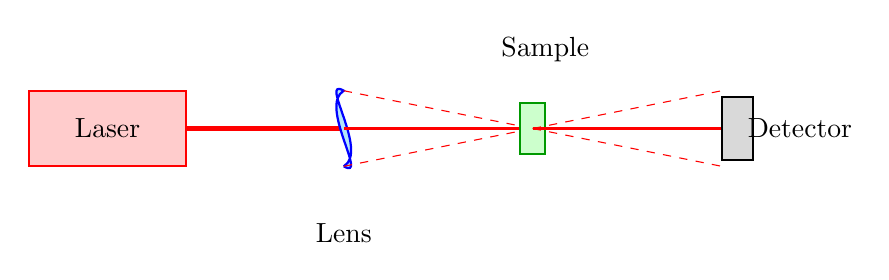
\begin{tikzpicture}[scale=0.8]
        % Laser source
        \draw[fill=red!20, draw=red, thick] (0, 0) rectangle (2.5, 1.2) node[midway] {Laser};
        \draw[red, line width=1.5pt] (2.5, 0.6) -- (5.0, 0.6); % beam before lens

        % Lens representation
        \draw[fill=cyan!30, draw=blue, thick] (5.0, 0) to[out=30, in=150] (5.0, 1.2) to[out=-150, in=-30] (5.0, 0) node[below=0.6cm] {Lens};

        % Focused beam converging to focal point
        \draw[red, line width=1.0pt] (5.0, 0.6) -- (8.0, 0.6);
        \draw[red, dashed] (5.0, 1.2) -- (8.0, 0.6);
        \draw[red, dashed] (5.0, 0) -- (8.0, 0.6);

        % Sample at focal point
        \draw[fill=green!20, draw=green!60!black, thick] (7.8, 0.2) rectangle (8.2, 1.0) node[above=0.4cm] {Sample};

        % Diverging beam after focal point
        \draw[red, dashed] (8.0, 0.6) -- (11.0, 1.2);
        \draw[red, dashed] (8.0, 0.6) -- (11.0, 0);
        \draw[red, line width=1.0pt] (8.0, 0.6) -- (11.0, 0.6);

        % Detector
        \draw[fill=gray!30, draw=black, thick] (11.0, 0.1) rectangle (11.5, 1.1) node[midway, right] {Detector};
    \end{tikzpicture}
    \caption{Schematic representation of the single-lens closed-aperture Z-scan configuration.}
    \label{fig:optical_schematic}
\end{figure}

\subsection{Circuit Diagram Example}
An example electronics circuit configuration for the detector amplification stage using \textsf{circuitikz} is shown in Figure \ref{fig:amplifier_circuit}:

\begin{figure}[H]
    \centering
    \begin{circuitikz}[scale=0.8]
        \draw (0,0) node[op amp] (opamp) {}
        (opamp.-) -- (-1.5,0.5) to[R, l=$R_1$] (-3,0.5) node[ground] {}
        (opamp.+) -- (-1.5,-0.5) to[empty photodiode, l=$D_{in}$] (-3,-0.5) node[ground] {}
        (opamp.-) -- (-1.5,0.5) -- (-1.5,2) to[R, l=$R_f$] (1.5,2) -| (opamp.out)
        (opamp.out) -- (1.5,0) node[right] {$V_{out}$};
    \end{circuitikz}
    \caption{Photodiode transimpedance amplifier schematic circuit diagram.}
    \label{fig:amplifier_circuit}
\end{figure}

\subsection{Analysis Code Script}
We use the following Python script to calculate the normalized transmission profile:
\begin{lstlisting}[style=pythonstyle, caption={Python routine for processing closed-aperture Z-scan values.}, label={lst:zscan_python}]
import numpy as np

def calculate_transmission(z, delta_phi):
    """
    Calculates normalized transmission for a third-order
    non-linear refractive index change.
    """
    x = z / 1.0 # normalized z coordinate
    transmission = 1 + (4 * delta_phi * x) / ((x**2 + 9) * (x**2 + 1))
    return transmission

# Sample coordinate generation
z_values = np.linspace(-5, 5, 100)
trans = calculate_transmission(z_values, delta_phi=0.5)
print("Peak transmission calculated at normalized position.")
\end{lstlisting}
